%!TEX root = ../proteoform_suite_manual.tex
%---------------------------------------------------------------------
%	LOAD DECONVOLUTION RESULTS
%---------------------------------------------------------------------

\section{Load Results: Standard}

This page is where the user loads in deconvolution results, top-down results, bottom-up results, and protein databases for the analysis on subsequent pages. On this page, chemical calibration can be performed on the deconvolution and top-down results (see \textbf{Calibration} section). Deconvolution and a top-down search can also be performed to generate deconvolution and top-down results (see \textbf{Deconvolution} and \textbf{Top-Down Search} sections, respectively). This section will describe the Load Results page for Standard analysis.

\subsection{Choose Analysis}

\begin{figure}[htbp]
\centering
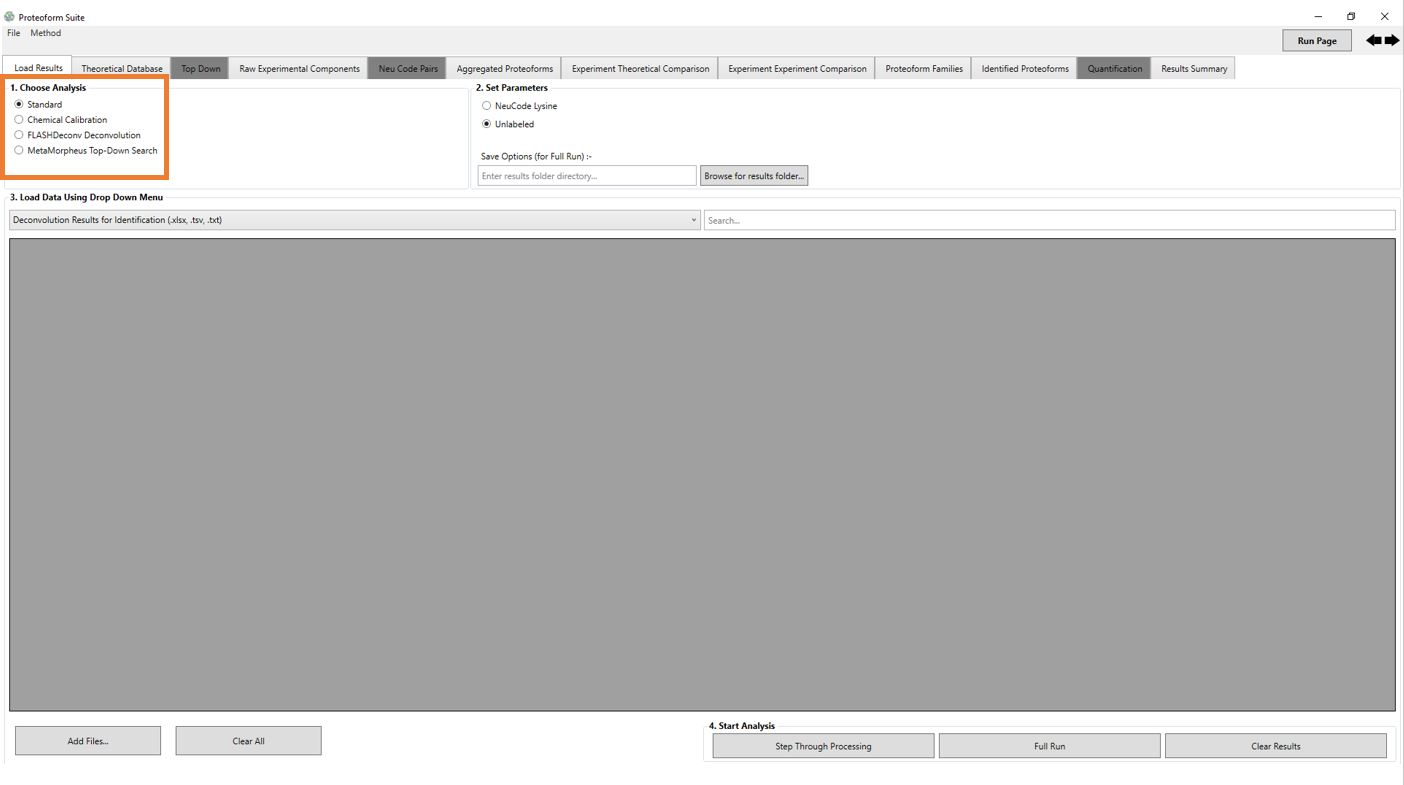
\includegraphics[scale=0.4]{figures/load_results_1.jpg}
\end{figure}

This option selects the type of analysis to perform.
\begin{itemize}
	\item Standard: load in results under standard before navigating through the different pages
	\item Chemical Calibration: calibrate mass and retention time of deconvolution and top-down results (see \textbf{Calibration} section)
	\item FLASHDeconv Deconvolution: deconvolute .mzML files (see \textbf {Deconvolution} section)
	\item MetaMorpheus Top-Down Search: search .mzML or .raw files for list of MS/MS identified proteoforms (see \textbf{Top-Down Search} section)
\end{itemize}

\pagebreak
\subsection{Set Parameters}

\begin{figure}[htbp]
\centering
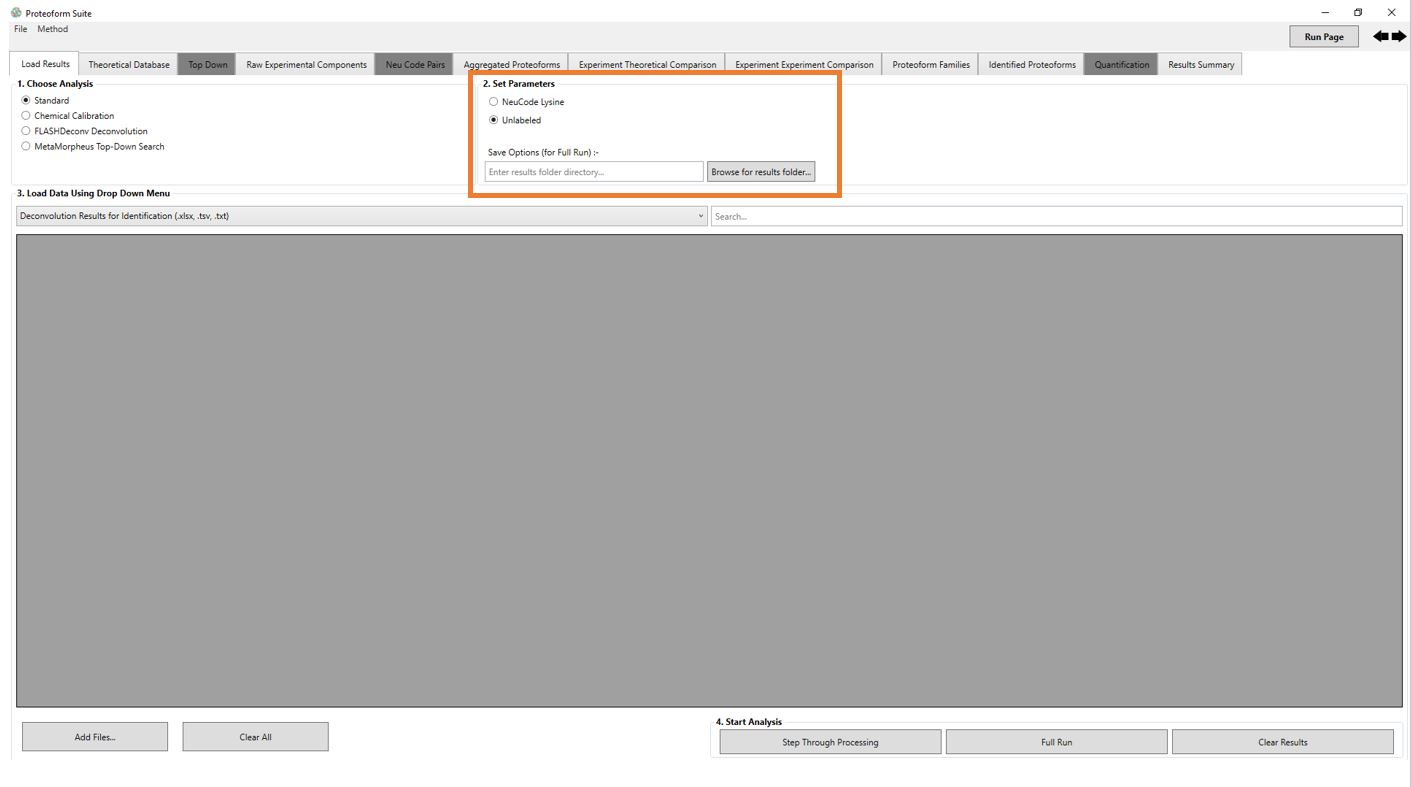
\includegraphics[scale=0.4]{figures/load_results_2.jpg}
\end{figure}

\begin{itemize}
	\item NeuCode Lysine: select if cell culture was performed with heavy and light NeuCode lysine tags 
	\item Unlabeled : select if no labeling was utilized (typical)
	\item Save Options: for full-run of a method .xml file (see below), select a file path to output results
\end{itemize}

\subsection{Load Data Using Drop Down Menu}

\begin{figure}[htbp]
\centering
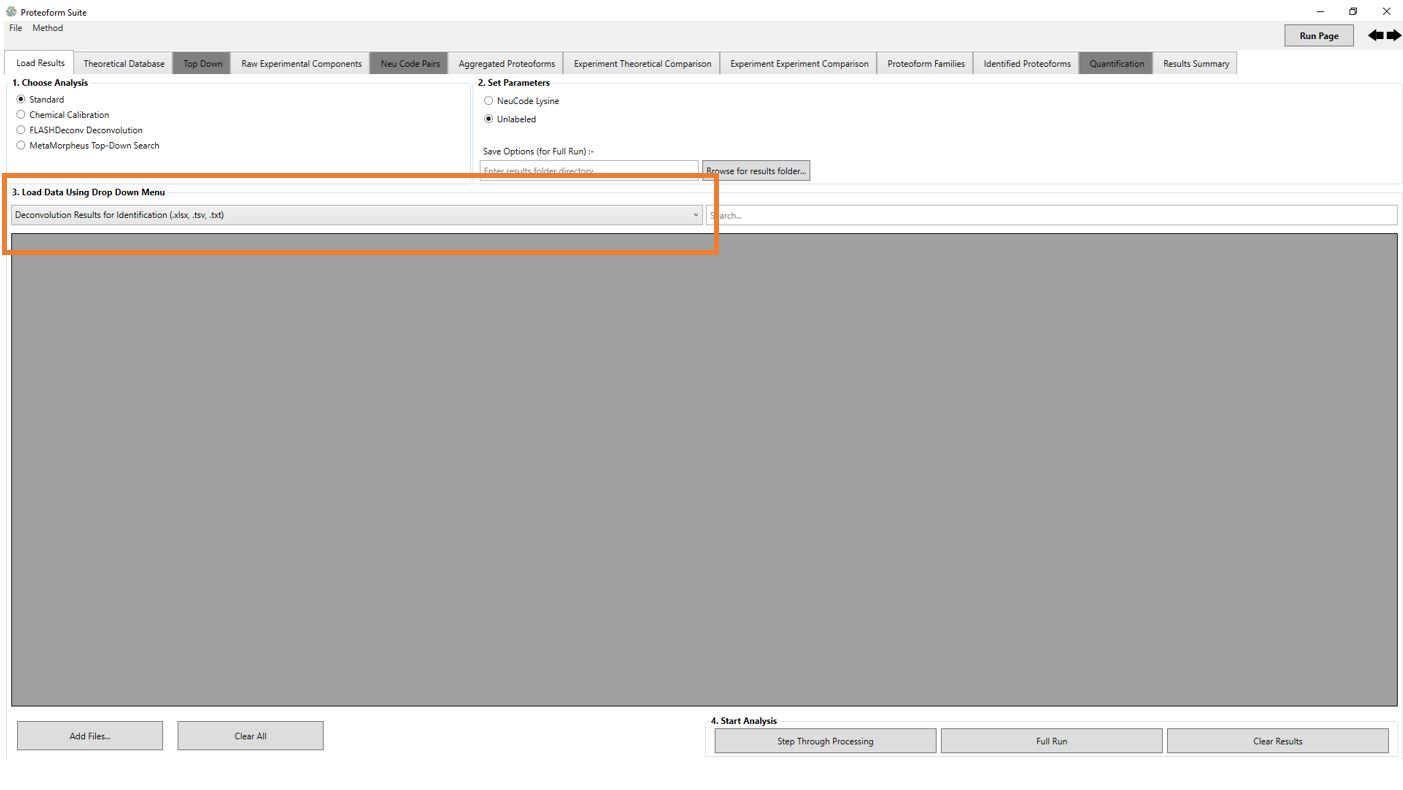
\includegraphics[scale=0.4]{figures/load_results_3.jpg}
\end{figure}

\begin{itemize}
	\item Drop down menu: Change file type to be added by selecting an item in the drop down box. Each file type is described below. 
	\item Add Files...: add files of the type selected in the drop down box
	\item Clear All: clear files of the type selected in the drop down box
\end{itemize}
\pagebreak
\subsection{Deconvolution Results for Identification}

Results from deconvolution of MS1 spectra, \textit{i.e.}, observed proteoform masses. These deconvolution results will be used to identify proteoforms by intact-mass analysis. There are three options for deconvolution results (see \textbf{Deconvolution} section):

\begin{itemize}
	\item Results from Thermo Deconvolution 4.0 (.xlsx)
	\item Results from FLASHDeconv (.tsv)
	\item A three column tab-separated .tsv or .txt file with columns mass, intensity, retention time
\end{itemize}

There is the option to label the Biological Replicate, Fraction, Technical Replicate, and Condition for each file. To change one of these labels for a single file, click the appropriate cell in the table. To change the label for more than one file or cell, select the cells you would like to change the label for, right click your mouse, enter a label, click Okay. 

\subsection{Deconvolution Results for Quantification}

It is only necessary to enter deconvolution results for quantification if you plan to perform a quantitative analysis of proteoform abundance changes between two conditions (see \textbf{Quantification} section). Results from deconvolution of MS1 spectra, \textit{i.e.}, observed proteoform masses. The proteoform intensity values in these deconvolution results will be used to quantify proteoforms.\supercite{Cesnik2018,Schaffer2018} These results files can be the same or different than the deconvolution results for identification.  There are three options for deconvolution results (see \textbf{Deconvolution} section):

\begin{itemize}
	\item Results from Thermo Deconvolution 4.0 (.xlsx)
	\item Results from FLASHDeconv (.tsv)
	\item A three column tab-separated .tsv or .txt file with columns mass, intensity, retention time
\end{itemize}

To perform a quantification analysis, it is necessary to label the Biological Replicate, Fraction, Technical Replicate, and Condition for each file. The change one of these labels for a single file, click the appropriate cell in the table. To change the label for more than one file or cell, select the cells you would like to change the label for, right click your mouse, enter a label, click Okay. 

\subsection{Protein Databases}

Download a protein database from UniProt (\url{https://www.uniprot.org/proteomes/}). It is recommended to use the Reviewed entries only. A database from MetaMorpheus generated from a bottom-up search and the global post-translational modification discovery strategy (G-PTM-D) can also be utilized.\supercite{Dai2017,Dai2019} Check the contaminant column if the database is a contaminant database. There are two options for protein databases:
\begin{itemize}
\item .xml or .xml.gz: contains annotated PTM information and subsequences
\item .fasta: option to include isoforms when downloaded
\end{itemize}

\subsection{Top-Down Hit Results}

Results from a top-down search of MS/MS spectra, \textit{i.e.}, proteoform identifications. There are two options for top-down results (see \textbf{Top-Down Search} section):
\begin{itemize}
	\item Results from TDPortal (.xlsx)
	\item Results from MetaMorpheus (.psmtsv)
\end{itemize} 

\subsection{MetaMorpheus Bottom-Up Unique Peptides}

Results from a bottom-up search of MS/MS spectra, \textit{i.e.}, peptide identifications.\supercite{Schaffer2020} Download a release of MetaMorpheus and run a bottom-up search (\url{https://github.com/smith-chem-wisc/MetaMorpheus/releases}). In the results folder of the search, load the AllPeptides.psmtsv file. 

\pagebreak
\subsection{Start Analysis}

\begin{figure}[h]
\centering
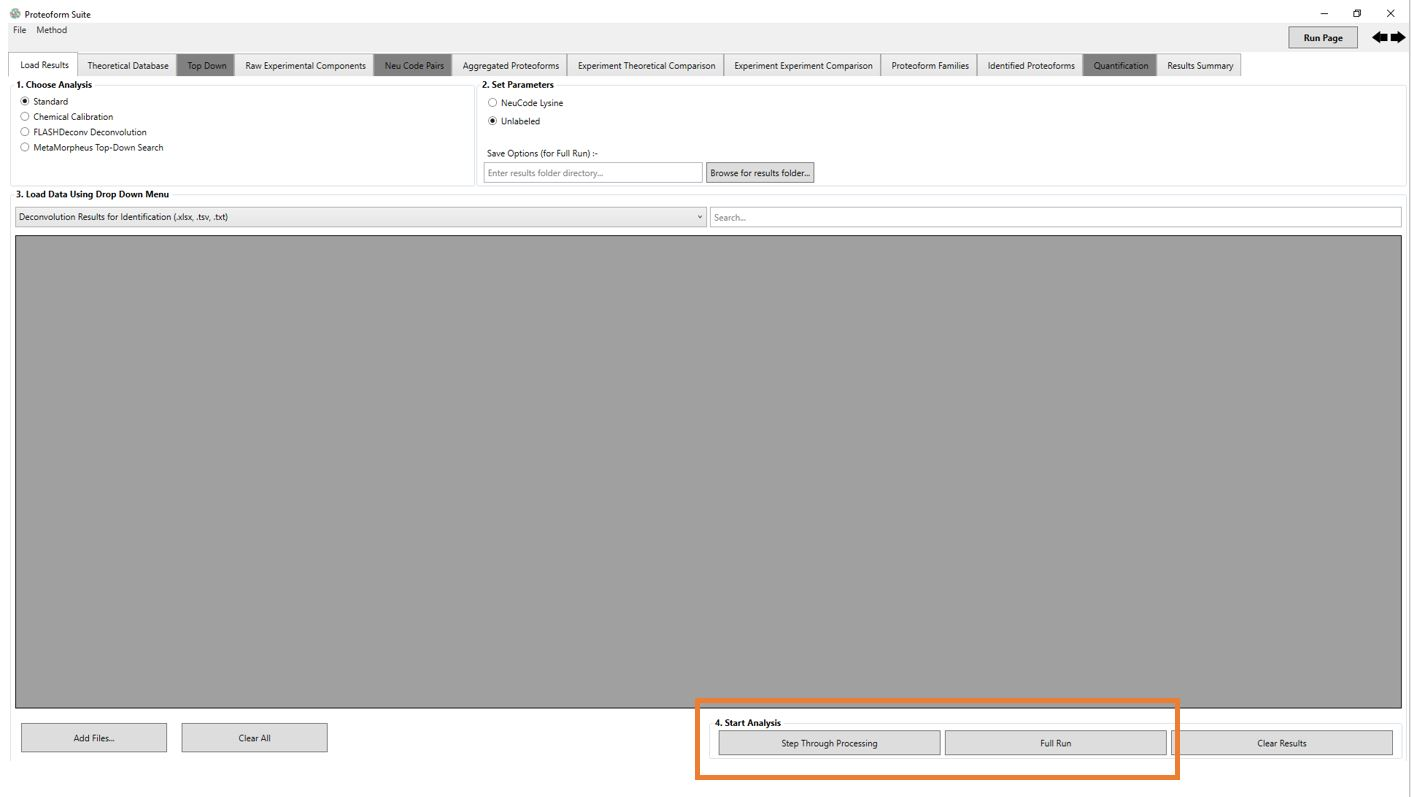
\includegraphics[scale=0.4]{figures/load_results_4.jpg}
\end{figure}

\begin{itemize}
	\item Step Through Processing button: instructions display on how to step through different pages
	\item Full Run button: load in a method .xml or use preset defaults to automatically perform a full run through analysis
	\item Clear Results button: clear all files in the file table
\end{itemize}
